\documentclass{ximera}

\title{CoCalc}

\begin{document}
\begin{abstract}
CoCalc is a way for a new author to publish.
\end{abstract}
\maketitle

To publish your work to the internet, you will need a computer that
can run our tools. The developers of Ximera use \link[Arch
  Linux]{http://www.archlinux.org/}, but we believe that to be too
difficult for the new user. Instead, we suggest you use
\link[CoCalc]{http://cocalc.com/}.



\section{Using your CoCalc account}


Once you have a CoCalc account, you will need to start a new project

\begin{image}
  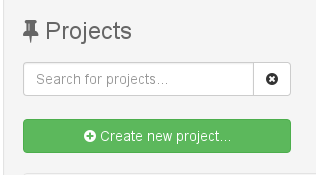
\includegraphics{createNewProject.png}
\end{image}

And when you create this new project, give it a Title, and a
Description. This project \textbf{must} have internet access.
\begin{image}
  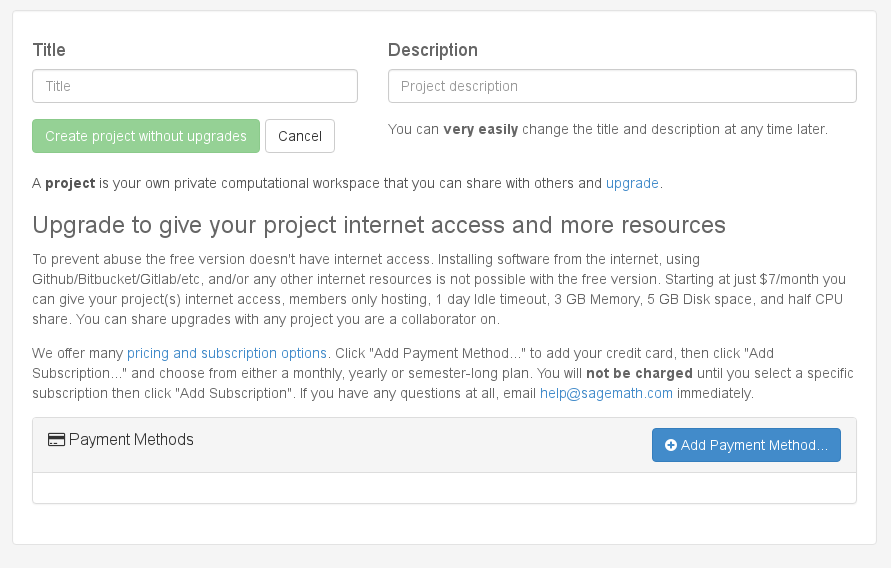
\includegraphics{internet.png}
\end{image}
Now you will need to add a terminal to your CoCalc account, click on
\begin{image}
  
\includegraphics{create.png}
\end{image}
and select ``Terminal.'' 
\begin{image}
  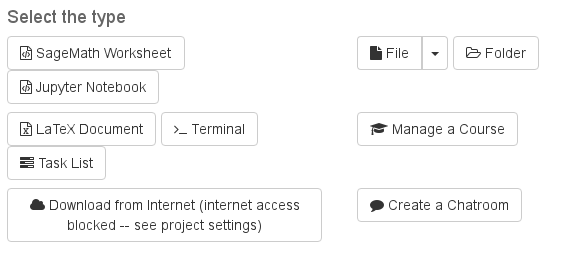
\includegraphics{type.png}
\end{image}
After a few seconds, a window will appear
\begin{image}
  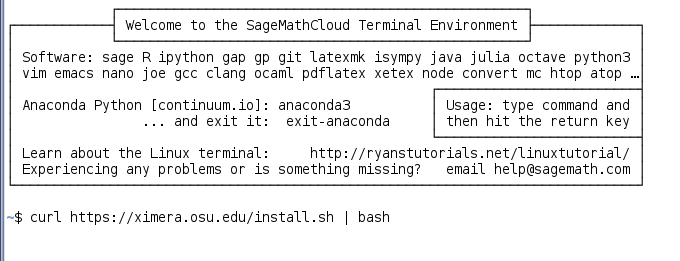
\includegraphics{typingCurl.png}
\end{image}
Then run the two commands
\begin{verbatim}
curl -OL http://xandbox.github.io/cocalc/install.sh
source install.sh

\end{verbatim}
This will install all the required tools (like the Ximera class file,
the `xake' build tool to compile and publish to the server, and mutool
for rasterizing graphics).


\subsection{Editing existing activity files}

\begin{enumerate}

\item Click on ``Files" to view the files that have been downloaded into your project.
\item Choose the directory ``xandbox" from the list of files. If you are working on your own computer, ``xandbox'' could be any directory.
\item Choose ``first.tex"
\item Make some edits and click ``Save."
\item Click on the terminal in your project.
\item At this point you need to set-up a git repository. This is not difficult, but it is dependent on what you name your git repository. See \link[this]{https://help.github.com/articles/creating-a-new-repository/}.
\item Now you will want to clone your repo into your xandbox directory.
\item You'll need to \verb!pull! your new repo. Move ``first.tex'' into your repo. 
\item Type \verb!git add first.tex! to stage the changes you've made to the first.tex file.
\item Type \verb!git commit -m "My first edit"! to commit the staged changes.
\item Type \verb!xake name! followed by a space and then a short lowercase name for your xandbox.  This could be your first name, for instance.  The name you choose must be globally unique, so be creative!  For instance, \verb!xake name turnloon! is what I will choose.
\item Type \verb!xake bake! to compile your first.tex into an html file.  If you run into errors, you can go back to your first.tex file and make additional edits.
\item Type \verb!xake frost! to create a publication commit on top of your source commit.
\item Type \verb!xake serve! to share your content with the world.  For instance, my content will appear at https://ximera.osu.edu/turnloon/first
\end{enumerate}

\subsection{Stuck?}

If you are stuck, please contact us at \texttt{ximera@math.osu.edu} to get help.



\end{document}
